\documentclass[a4paper,14pt]{article}
\usepackage[utf8]{inputenc}
\usepackage[margin=1in]{geometry}
\usepackage{caption}
\usepackage{multirow,array,varwidth}
\usepackage{lscape}
\usepackage{hyperref}
\usepackage{graphicx}

%opening
\title{The BAW Instruction Set Manual}
\author{Bryant Herren, Wesley Ring, Austin Waddell}
\date{}

\begin{document}

\newcommand\DescEntry[1]{%
  \multirow{1}*{%
    \begin{varwidth}{13em}% --- or minipage, if you prefer a fixed width
    \flushright #1%
    \end{varwidth}}}

\newcommand\Tstrut{\rule{0pt}{2.6ex}}       % "top" strut
\newcommand\Bstrut{\rule[-0.9ex]{0pt}{0pt}} % "bottom" strut
\newcommand{\TBstrut}{\Tstrut\Bstrut} % top&bottom struts
    
\null  % Empty line
\nointerlineskip  % No skip for prev line
\vfill
\let\snewpage \newpage
\let\newpage \relax
\maketitle
\let \newpage \snewpage
\vfill 
\newpage

{\hypersetup{linktoc=all,hidelinks}
\tableofcontents
}
\newpage

\section{Introduction}
BAW is the instruction set for a floating point co-processor designed in ECGR 3183 at the University of North Carolina at Charlotte. The co-processor was implemented with a single-cycle architecture, and a pipelined architecture. For the pipelined architecture, two branch prediction algorithms were implemented (1 static and 1 dynamic) as well as no branch prediction.
\newline\newline
Provided in this document:
\begin{itemize}
    \setlength{\parskip}{0pt}
    \setlength{\itemsep}{0pt plus 1pt}
    \item The complete ISA
    \item Architecture and controller design (units, diagrams, etc)
    \item VHDL simulation
    \item Performance results and discussion for pipelined vs. unpipelined approaches
\end{itemize}


\subsection{System Parameters}
\begin{itemize}
    \setlength{\parskip}{0pt}
    \setlength{\itemsep}{0pt plus 1pt}
    \item 32 bits per instruction/register
    \item Data is stored using IEEE single-precision floating point numbers.
    \item Register file has 16 registers
    \item Timings:
    \begin{itemize}
        \setlength{\parskip}{0pt}
        \item Clock cycle (pipelined): 100ns
        \item Register Read/Write: 100ns
        \item Memory Read/Write: 300ns
        \item Single ALU Op: 200ns
    \end{itemize}
\end{itemize}

\subsection{Memory}
The system includes a data memory addressed 0-1023 and 16 Floating Point registers (Referenced as X0-X15). Each memory location and register uses a 32-bit value. The simulation can read an input file containing the operational parameters, code, and memory contents (there is an assembler).
\subsection{Additional Features}
\begin{itemize}
    \setlength{\parskip}{0pt}
    \setlength{\itemsep}{0pt plus 1pt}
    \item FP Multiply by -1, 1, or 0 takes 1 cycle
    \item FP Multiply by power of 2 takes 2 cycles
    \item Condition Codes:
    \begin{itemize}
        \setlength{\parskip}{0pt}
        \setlength{\itemsep}{0pt plus 1pt}
        \item Z - Zero
        \item N - Negative
        \item V - Overflow
        \item C - Carry
        \item E - Error (domain errors, etc.)
    \end{itemize}
    \item All condition codes are set as needed on arithmetic operations
    \item The round, ceiling, and floor functions would round up to the nearest integer, expressing the result in floating point format.
\end{itemize}

\section{ISA}
\subsection{Introduction}
The ISA is based off of the ARMv8 / LEGv8 ISA. As a result, there will likely be similarities.

\subsection{Instruction Format}
There are four instruction formats: Register (R), Data (D), Immediate (I), and Branch (B). 
All processor instructions are 32 bits wide. Table \ref{table:format_descriptions} Contains information about the specific instruction formats.
\newline
\newline
Notes:
\begin{enumerate}
    \item The Opcode is 8 bits long, allowing it to be easily read in hex format. This also allows additional instructions to be added in the future.
    \item The remaining three bits of each instruction format are not used. This allows for the addition of specialized registers (zero register, etc.) if needed.
\end{enumerate}

\begin{table}
\centering
\caption{Instruction Format Descriptions}
\label{table:format_descriptions}
\begin{tabular}{| l | p{7cm} | l |}
\hline
Format & Description & Example \\ \hline
R (Register) & An instruction whose inputs and outputs are both registers & ADD X9, X21, X9 \\ \hline
D (Data) & An instruction used when fetching or placing data in memory & LOAD X9, {[}X22, \#64{]} \\ \hline
I (Immediate) & An instruction that carries specific additional data & POW X9, \#15 \\ \hline
B (Branch) & An instruction that deals with changing the location of the PC directly & PC $\leftarrow$  M[Ri] \\ \hline
\end{tabular}
\end{table}

Please see Table \ref{table:instruction_formats} for specific information on the Instruction Formats.

\begin{landscape}
\begin{table}
\setlength\tabcolsep{4pt}
\caption{Instruction Formats}
\label{table:instruction_formats}
\begin{tabular}{|l|l|l|l|l|l|l|l|l|llllllllllll|l|l|l|l|l|l|l|l|l|l|l|l|l|}
\hline
\multicolumn{1}{|r|}{Instruction Format} & 0 & 1 & 2 & 3 & 4 & 5 & 6 & 7 & \multicolumn{1}{l|}{8} & \multicolumn{1}{l|}{9} & \multicolumn{1}{l|}{10} & \multicolumn{1}{l|}{11} & \multicolumn{1}{l|}{12} & \multicolumn{1}{l|}{13} & \multicolumn{1}{l|}{14} & \multicolumn{1}{l|}{15} & \multicolumn{1}{l|}{16} & \multicolumn{1}{l|}{17} & \multicolumn{1}{l|}{18} & 19 & 20 & 21 & 22 & 23 & 24 & 25 & 26 & 27 & 28 & 29 & 30 & 31 & 32 \\ \hline

R (Register) & \multicolumn{8}{l|}{Opcode (8 bits)} & \multicolumn{5}{l|}{Rm (5 bit)} & \multicolumn{7}{l|}{Empty (7 bit)} & \multicolumn{5}{l|}{Rn (5 bit)} & \multicolumn{5}{l|}{Rd (5 bit)} & \multicolumn{3}{l|}{\multirow{3}{*}{\begin{tabular}[c]{@{}l@{}}Empty \\ \\ (3 bit)\end{tabular}}} \\ \cline{1-31}

D (Data) & \multicolumn{8}{l|}{Opcode (8 bits)} & \multicolumn{10}{l|}{Address (9 bit)} & \multicolumn{2}{l|}{op2 (2 bit)} & \multicolumn{5}{l|}{Rn (5 bit)} & \multicolumn{5}{l|}{Rd (5 bit)} & \multicolumn{3}{l|}{} \\ \cline{1-31}

I (Immediate) & \multicolumn{8}{l|}{Opcode (8 bits)} & \multicolumn{12}{l|}{Immediate Data (11 bit)} & \multicolumn{5}{l|}{Rn (5 bit)} & \multicolumn{5}{l|}{Rd (5 bit)} & \multicolumn{3}{l|}{} \\ \cline{1-31}

B (Branch) & \multicolumn{8}{l|}{Opcode (8 bits)} & \multicolumn{17}{l|}{Address (16 bits)} &  \multicolumn{5}{l|}{Rd (5 bit)} & \multicolumn{3}{l|}{} \\ \hline
\end{tabular}
\end{table}
\end{landscape}

\subsection{Instructions}




%=======================================

\subsubsection{Set}
\begin{table}[!h]
\centering
\caption*{SET}
\begin{tabular}{llllll}
ASM & Opcode & Format & Description & Operation & ALU Cycles \\ \hline
\multicolumn{1}{|c|}{SET} & \multicolumn{1}{c|}{00000001} & \multicolumn{1}{c|}{I} & \DescEntry{Sets Ri to given floating point value} \vline & \multicolumn{1}{c|}{Ri $\leftarrow$  FPvalue} & \multicolumn{1}{c|}{1} \TBstrut \\[1em] \hline
\end{tabular}
\end{table}

\begin{itemize}
    \setlength{\parskip}{0pt}
    \setlength{\itemsep}{0pt plus 1pt}
    \setlength{\itemindent}{-4mm}
    \item[] \textbf{ASM Example:} SET Ri, \#FPvalue
\end{itemize}
\begin{itemize}
    \setlength{\parskip}{0pt}
    \setlength{\itemsep}{0pt plus 1pt}
    \setlength{\itemindent}{7mm}
    \item [\textbf{Flags}]
    \item Zero
    \item Negitive
\end{itemize}

\subsubsection{Load}
\begin{table}[!h]
\centering
\caption*{LOD}
\begin{tabular}{llllll}
ASM & Opcode & Format & Description & Operation & ALU Cycles \\ \hline
\multicolumn{1}{|c|}{LOD} & \multicolumn{1}{c|}{00000010} & \multicolumn{1}{c|}{D} & \DescEntry{Copies Rj from memory and into Ri} \vline & \multicolumn{1}{c|}{Ri $\leftarrow$  M[Rj]} & \multicolumn{1}{c|}{1} \TBstrut \\[1em] \hline
\end{tabular}
\end{table}

\begin{itemize}
    \setlength{\parskip}{0pt}
    \setlength{\itemsep}{0pt plus 1pt}
    \setlength{\itemindent}{-4mm}
    \item[] \textbf{ASM Example:} LOD Ri, Rj
\end{itemize}
\begin{itemize}
    \setlength{\parskip}{0pt}
    \setlength{\itemsep}{0pt plus 1pt}
    \setlength{\itemindent}{7mm}
    \item [\textbf{Flags}]
    \item Zero
    \item Negitive
\end{itemize}

\subsubsection{Store}
\begin{table}[!h]
\centering
\caption*{STR}
\begin{tabular}{llllll}
ASM & Opcode & Format & Description & Operation & ALU Cycles \\ \hline
\multicolumn{1}{|c|}{STR} & \multicolumn{1}{c|}{00000011} & \multicolumn{1}{c|}{D} & \DescEntry{Copies data from register Rj into memory} \vline & \multicolumn{1}{c|}{M[Ri] $\leftarrow$  Rj} & \multicolumn{1}{c|}{1} \TBstrut \\[1em] \hline
\end{tabular}
\end{table}

\begin{itemize}
    \setlength{\parskip}{0pt}
    \setlength{\itemsep}{0pt plus 1pt}
    \setlength{\itemindent}{-4mm}
    \item[] \textbf{ASM Example:} STR Ri, Rj
\end{itemize}
\begin{itemize}
    \setlength{\parskip}{0pt}
    \setlength{\itemsep}{0pt plus 1pt}
    \setlength{\itemindent}{7mm}
    \item [\textbf{Flags}]
    \item None
\end{itemize}

\newpage

\subsubsection{Move}
\begin{table}[!h]
\centering
\caption*{MOV}
\begin{tabular}{llllll}
ASM & Opcode & Format & Description & Operation & ALU Cycles \\ \hline
\multicolumn{1}{|c|}{MOV} & \multicolumn{1}{c|}{00000100} & \multicolumn{1}{c|}{R} & \DescEntry{Moves the value of Rj to Ri, deleting the original} \vline & \multicolumn{1}{c|}{Ri $\leftarrow$  Rj} & \multicolumn{1}{c|}{1} \TBstrut \\[1em] \hline
\end{tabular}
\end{table}

\begin{itemize}
    \setlength{\parskip}{0pt}
    \setlength{\itemsep}{0pt plus 1pt}
    \setlength{\itemindent}{-4mm}
    \item[] \textbf{ASM Example:} MOV Ri, Rj
\end{itemize}
\begin{itemize}
    \setlength{\parskip}{0pt}
    \setlength{\itemsep}{0pt plus 1pt}
    \setlength{\itemindent}{7mm}
    \item [\textbf{Flags}]
    \item Zero
    \item Negitive
\end{itemize}

\subsubsection{Add}
\begin{table}[!h]
\centering
\caption*{ADD}
\begin{tabular}{llllll}
ASM & Opcode & Format & Description & Operation & ALU Cycles \\ \hline
\multicolumn{1}{|c|}{ADD} & \multicolumn{1}{c|}{00000101} & \multicolumn{1}{c|}{R} & \DescEntry{Adds Rj and Rk into Ri} \vline & \multicolumn{1}{c|}{Ri $\leftarrow$  Rj + Rk} & \multicolumn{1}{c|}{3} \TBstrut \\[1em] \hline
\end{tabular}
\end{table}

\begin{itemize}
    \setlength{\parskip}{0pt}
    \setlength{\itemsep}{0pt plus 1pt}
    \setlength{\itemindent}{-4mm}
    \item[] \textbf{ASM Example:} ADD Ri, Rj, Rk
\end{itemize}
\begin{itemize}
    \setlength{\parskip}{0pt}
    \setlength{\itemsep}{0pt plus 1pt}
    \setlength{\itemindent}{7mm}
    \item [\textbf{Flags}]
    \item Zero
    \item Negitive
    \item Overflow
    \item Carry
\end{itemize}

\subsubsection{Subtract}
\begin{table}[!h]
\centering
\caption*{SUB}
\begin{tabular}{llllll}
ASM & Opcode & Format & Description & Operation & ALU Cycles \\ \hline
\multicolumn{1}{|c|}{SUB} & \multicolumn{1}{c|}{00000110} & \multicolumn{1}{c|}{R} & \DescEntry{Subtrcts Rk from Rj into Ri} \vline & \multicolumn{1}{c|}{Ri $\leftarrow$  Rj – Rk} & \multicolumn{1}{c|}{3} \TBstrut \\[1em] \hline
\end{tabular}
\end{table}

\begin{itemize}
    \setlength{\parskip}{0pt}
    \setlength{\itemsep}{0pt plus 1pt}
    \setlength{\itemindent}{-4mm}
    \item[] \textbf{ASM Example:} SUB Ri, Rj, Rk
\end{itemize}
\begin{itemize}
    \setlength{\parskip}{0pt}
    \setlength{\itemsep}{0pt plus 1pt}
    \setlength{\itemindent}{7mm}
    \item [\textbf{Flags}]
    \item Zero
    \item Negitive
    \item Overflow
    \item Carry
\end{itemize}

\newpage

\subsubsection{Negate}
\begin{table}[!h]
\centering
\caption*{NEG}
\begin{tabular}{llllll}
ASM & Opcode & Format & Description & Operation & ALU Cycles \\ \hline
\multicolumn{1}{|c|}{NEG} & \multicolumn{1}{c|}{00000111} & \multicolumn{1}{c|}{R} & \DescEntry{Sets Ri to the Opposite of Rj} \vline & \multicolumn{1}{c|}{Ri $\leftarrow$  -Rj} & \multicolumn{1}{c|}{1} \TBstrut \\[1em] \hline
\end{tabular}
\end{table}

\begin{itemize}
    \setlength{\parskip}{0pt}
    \setlength{\itemsep}{0pt plus 1pt}
    \setlength{\itemindent}{-4mm}
    \item[] \textbf{ASM Example:} NEG Ri, Rj
\end{itemize}
\begin{itemize}
    \setlength{\parskip}{0pt}
    \setlength{\itemsep}{0pt plus 1pt}
    \setlength{\itemindent}{7mm}
    \item [\textbf{Flags}]
    \item Zero
    \item Negitive
\end{itemize}

\subsubsection{Multiply}
\begin{table}[!h]
\centering
\caption*{MUL}
\begin{tabular}{llllll}
ASM & Opcode & Format & Description & Operation & ALU Cycles \\ \hline
\multicolumn{1}{|c|}{MUL} & \multicolumn{1}{c|}{00001000} & \multicolumn{1}{c|}{R} & \DescEntry{Multiplies Rj and Rk into Ri} \vline & \multicolumn{1}{c|}{Ri $\leftarrow$  Rj * Rk} & \multicolumn{1}{c|}{5} \TBstrut \\[1em] \hline
\end{tabular}
\end{table}

\begin{itemize}
    \setlength{\parskip}{0pt}
    \setlength{\itemsep}{0pt plus 1pt}
    \setlength{\itemindent}{-4mm}
    \item[] \textbf{ASM Example:} MUL Ri, Rj, Rk
\end{itemize}
\begin{itemize}
    \setlength{\parskip}{0pt}
    \setlength{\itemsep}{0pt plus 1pt}
    \setlength{\itemindent}{7mm}
    \item [\textbf{Flags}]
    \item Zero
    \item Negitive
    \item Overflow
    \item Carry
\end{itemize}

\subsubsection{Divide}
\begin{table}[!h]
\centering
\caption*{DIV}
\begin{tabular}{llllll}
ASM & Opcode & Format & Description & Operation & ALU Cycles \\ \hline
\multicolumn{1}{|c|}{DIV} & \multicolumn{1}{c|}{00001001} & \multicolumn{1}{c|}{R} & \DescEntry{Divides Rj by Rk into Ri} \vline & \multicolumn{1}{c|}{Ri $\leftarrow$  Rj / Rk} & \multicolumn{1}{c|}{8} \TBstrut \\[1em] \hline
\end{tabular}
\end{table}

\begin{itemize}
    \setlength{\parskip}{0pt}
    \setlength{\itemsep}{0pt plus 1pt}
    \setlength{\itemindent}{-4mm}
    \item[] \textbf{ASM Example:} DIV Ri, Rj, Rk
\end{itemize}
\begin{itemize}
    \setlength{\parskip}{0pt}
    \setlength{\itemsep}{0pt plus 1pt}
    \setlength{\itemindent}{7mm}
    \item [\textbf{Flags}]
    \item Zero
    \item Negitive
    \item Overflow
    \item Carry
    \item Error - divide by zero
\end{itemize}

\newpage

\subsubsection{Floor}
\begin{table}[!h]
\centering
\caption*{FLR}
\begin{tabular}{llllll}
ASM & Opcode & Format & Description & Operation & ALU Cycles \\ \hline
\multicolumn{1}{|c|}{FLR} & \multicolumn{1}{c|}{00001010} & \multicolumn{1}{c|}{R} & \DescEntry{Sets Ri to the floor of Rj} \vline & \multicolumn{1}{c|}{Ri $\leftarrow$  $\lfloor$ Rj$\rfloor$ } & \multicolumn{1}{c|}{1} \TBstrut \\[1em] \hline
\end{tabular}
\end{table}

\begin{itemize}
    \setlength{\parskip}{0pt}
    \setlength{\itemsep}{0pt plus 1pt}
    \setlength{\itemindent}{-4mm}
    \item[] \textbf{ASM Example:} FLR Ri, Rj
\end{itemize}
\begin{itemize}
    \setlength{\parskip}{0pt}
    \setlength{\itemsep}{0pt plus 1pt}
    \setlength{\itemindent}{7mm}
    \item [\textbf{Flags}]
    \item Zero
    \item Negitive
\end{itemize}

\subsubsection{Ceiling}
\begin{table}[!h]
\centering
\caption*{CEL}
\begin{tabular}{llllll}
ASM & Opcode & Format & Description & Operation & ALU Cycles \\ \hline
\multicolumn{1}{|c|}{CEL} & \multicolumn{1}{c|}{00001011} & \multicolumn{1}{c|}{R} & \DescEntry{Sets Ri to the ceil of Rj} \vline & \multicolumn{1}{c|}{Ri $\leftarrow$  $\lceil$ Rj$\rceil$ } & \multicolumn{1}{c|}{1} \TBstrut \\[1em] \hline
\end{tabular}
\end{table}

\begin{itemize}
    \setlength{\parskip}{0pt}
    \setlength{\itemsep}{0pt plus 1pt}
    \setlength{\itemindent}{-4mm}
    \item[] \textbf{ASM Example:} CEL Ri, Rj
\end{itemize}
\begin{itemize}
    \setlength{\parskip}{0pt}
    \setlength{\itemsep}{0pt plus 1pt}
    \setlength{\itemindent}{7mm}
    \item [\textbf{Flags}]
    \item Zero
    \item Negitive
\end{itemize}

\subsubsection{Round}
\begin{table}[!h]
\centering
\caption*{RND}
\begin{tabular}{llllll}
ASM & Opcode & Format & Description & Operation & ALU Cycles \\ \hline
\multicolumn{1}{|c|}{RND} & \multicolumn{1}{c|}{00001100} & \multicolumn{1}{c|}{R} & \DescEntry{Sets Ri to Rj rounded to the nearest integer} \vline & \multicolumn{1}{c|}{Ri $\leftarrow$  round(Rj)} & \multicolumn{1}{c|}{1} \TBstrut \\[1em] \hline
\end{tabular}
\end{table}

\begin{itemize}
    \setlength{\parskip}{0pt}
    \setlength{\itemsep}{0pt plus 1pt}
    \setlength{\itemindent}{-4mm}
    \item[] \textbf{ASM Example:} RND Ri, Rj
\end{itemize}
\begin{itemize}
    \setlength{\parskip}{0pt}
    \setlength{\itemsep}{0pt plus 1pt}
    \setlength{\itemindent}{7mm}
    \item [\textbf{Flags}]
    \item Zero
    \item Negitive
\end{itemize}

\newpage

\subsubsection{Absolute Value}
\begin{table}[!h]
\centering
\caption*{ABS}
\begin{tabular}{llllll}
ASM & Opcode & Format & Description & Operation & ALU Cycles \\ \hline
\multicolumn{1}{|c|}{ABS} & \multicolumn{1}{c|}{00001101} & \multicolumn{1}{c|}{R} & \DescEntry{Sets Ri to the absolute value of Rj} \vline & \multicolumn{1}{c|}{Ri $\leftarrow$  | Rj |} & \multicolumn{1}{c|}{1} \TBstrut \\[1em] \hline
\end{tabular}
\end{table}

\begin{itemize}
    \setlength{\parskip}{0pt}
    \setlength{\itemsep}{0pt plus 1pt}
    \setlength{\itemindent}{-4mm}
    \item[] \textbf{ASM Example:} ABS Ri, Rj
\end{itemize}
\begin{itemize}
    \setlength{\parskip}{0pt}
    \setlength{\itemsep}{0pt plus 1pt}
    \setlength{\itemindent}{7mm}
    \item [\textbf{Flags}]
    \item Zero
\end{itemize}

\subsubsection{Minimum}
\begin{table}[!h]
\centering
\caption*{MIN}
\begin{tabular}{llllll}
ASM & Opcode & Format & Description & Operation & ALU Cycles \\ \hline
\multicolumn{1}{|c|}{MIN} & \multicolumn{1}{c|}{00001110} & \multicolumn{1}{c|}{R} & \DescEntry{Sets Ri to the minimum value between Rj and Rk} \vline & \multicolumn{1}{c|}{Ri $\leftarrow$  min( Rj, Rk)} & \multicolumn{1}{c|}{1} \TBstrut \\[1em] \hline
\end{tabular}
\end{table}

\begin{itemize}
    \setlength{\parskip}{0pt}
    \setlength{\itemsep}{0pt plus 1pt}
    \setlength{\itemindent}{-4mm}
    \item[] \textbf{ASM Example:} MIN Ri, Rj, Rk
\end{itemize}
\begin{itemize}
    \setlength{\parskip}{0pt}
    \setlength{\itemsep}{0pt plus 1pt}
    \setlength{\itemindent}{7mm}
    \item [\textbf{Flags}]
    \item Zero
    \item Negitive
\end{itemize}

\subsubsection{Maximum}
\begin{table}[!h]
\centering
\caption*{MAX}
\begin{tabular}{llllll}
ASM & Opcode & Format & Description & Operation & ALU Cycles \\ \hline
\multicolumn{1}{|c|}{MAX} & \multicolumn{1}{c|}{00001111} & \multicolumn{1}{c|}{R} & \DescEntry{Sets Ri to the maximum value between Rj and Rk} \vline & \multicolumn{1}{c|}{Ri $\leftarrow$  max( Rj, Rk)} & \multicolumn{1}{c|}{1} \TBstrut \\[1em] \hline
\end{tabular}
\end{table}

\begin{itemize}
    \setlength{\parskip}{0pt}
    \setlength{\itemsep}{0pt plus 1pt}
    \setlength{\itemindent}{-4mm}
    \item[] \textbf{ASM Example:} MAX Ri, Rj, Rk
\end{itemize}
\begin{itemize}
    \setlength{\parskip}{0pt}
    \setlength{\itemsep}{0pt plus 1pt}
    \setlength{\itemindent}{7mm}
    \item [\textbf{Flags}]
    \item Zero
    \item Negitive
\end{itemize}

\newpage

\subsubsection{Power}
\begin{table}[!h]
\centering
\caption*{POW}
\begin{tabular}{llllll}
ASM & Opcode & Format & Description & Operation & ALU Cycles \\ \hline
\multicolumn{1}{|c|}{POW} & \multicolumn{1}{c|}{00010000} & \multicolumn{1}{c|}{I} & \DescEntry{Sets Ri to Rj raised to some given integer power} \vline & \multicolumn{1}{c|}{Ri $\leftarrow$  Rj\textasciicircum integer\_value} & \multicolumn{1}{c|}{6} \TBstrut \\[1em] \hline
\end{tabular}
\end{table}

\begin{itemize}
    \setlength{\parskip}{0pt}
    \setlength{\itemsep}{0pt plus 1pt}
    \setlength{\itemindent}{-4mm}
    \item[] \textbf{ASM Example:} POW Ri, Rj, \#integer\_value
\end{itemize}
\begin{itemize}
    \setlength{\parskip}{0pt}
    \setlength{\itemsep}{0pt plus 1pt}
    \setlength{\itemindent}{7mm}
    \item [\textbf{Flags}]
    \item Zero
    \item Negitive
    \item Overflow
    \item Carry
\end{itemize}

\subsubsection{Exponent}
\begin{table}[!h]
\centering
\caption*{EXP}
\begin{tabular}{llllll}
ASM & Opcode & Format & Description & Operation & ALU Cycles \\ \hline
\multicolumn{1}{|c|}{EXP} & \multicolumn{1}{c|}{00010001} & \multicolumn{1}{c|}{R} & \DescEntry{Sets Ri to Rj exponentiated} \vline & \multicolumn{1}{c|}{Ri $\leftarrow$  e\textasciicircum Rj} & \multicolumn{1}{c|}{8} \TBstrut \\[1em] \hline
\end{tabular}
\end{table}

\begin{itemize}
    \setlength{\parskip}{0pt}
    \setlength{\itemsep}{0pt plus 1pt}
    \setlength{\itemindent}{-4mm}
    \item[] \textbf{ASM Example:} EXP Ri, Rj
\end{itemize}
\begin{itemize}
    \setlength{\parskip}{0pt}
    \setlength{\itemsep}{0pt plus 1pt}
    \setlength{\itemindent}{7mm}
    \item [\textbf{Flags}]
    \item Overflow
    \item Carry
\end{itemize}

\subsubsection{Square Root}
\begin{table}[!h]
\centering
\caption*{SQR}
\begin{tabular}{llllll}
ASM & Opcode & Format & Description & Operation & ALU Cycles \\ \hline
\multicolumn{1}{|c|}{SQR} & \multicolumn{1}{c|}{00010010} & \multicolumn{1}{c|}{R} & \DescEntry{Sets Ri to the square root of Rj} \vline & \multicolumn{1}{c|}{Ri $\leftarrow$  $\surd$ Rj} & \multicolumn{1}{c|}{8} \TBstrut \\[1em] \hline
\end{tabular}
\end{table}

\begin{itemize}
    \setlength{\parskip}{0pt}
    \setlength{\itemsep}{0pt plus 1pt}
    \setlength{\itemindent}{-4mm}
    \item[] \textbf{ASM Example:} SQR Ri, Rj
\end{itemize}
\begin{itemize}
    \setlength{\parskip}{0pt}
    \setlength{\itemsep}{0pt plus 1pt}
    \setlength{\itemindent}{7mm}
    \item [\textbf{Flags}]
    \item Zero
    \item Overflow
    \item Carry
    \item Error - complex domain
\end{itemize}

\newpage

\subsubsection{Branch (Uncond.)}
\begin{table}[!h]
\centering
\caption*{BRU}
\begin{tabular}{llllll}
ASM & Opcode & Format & Description & Operation & ALU Cycles \\ \hline
\multicolumn{1}{|c|}{BRU} & \multicolumn{1}{c|}{00010011} & \multicolumn{1}{c|}{B} & \DescEntry{Loads Ri from memory into PC} \vline & \multicolumn{1}{c|}{PC $\leftarrow$  M[Ri]} & \multicolumn{1}{c|}{1} \TBstrut \\[1em] \hline
\end{tabular}
\end{table}

\begin{itemize}
    \setlength{\parskip}{0pt}
    \setlength{\itemsep}{0pt plus 1pt}
    \setlength{\itemindent}{-4mm}
    \item[] \textbf{ASM Example:} BRU Ri
\end{itemize}
\begin{itemize}
    \setlength{\parskip}{0pt}
    \setlength{\itemsep}{0pt plus 1pt}
    \setlength{\itemindent}{7mm}
    \item [\textbf{Flags}]
    \item None
\end{itemize}

\subsubsection{Branch Zero}
\begin{table}[!h]
\centering
\caption*{BRZ}
\begin{tabular}{llllll}
ASM & Opcode & Format & Description & Operation & ALU Cycles \\ \hline
\multicolumn{1}{|c|}{BRZ} & \multicolumn{1}{c|}{00010100} & \multicolumn{1}{c|}{B} & \DescEntry{Sends the PC to a specific labeled line if Ri is zero} \vline & \multicolumn{1}{c|}{If (Ri == 0) PC $\leftarrow$  LABEL (line)} & \multicolumn{1}{c|}{3} \TBstrut \\[1em] \hline
\end{tabular}
\end{table}

\begin{itemize}
    \setlength{\parskip}{0pt}
    \setlength{\itemsep}{0pt plus 1pt}
    \setlength{\itemindent}{-4mm}
    \item[] \textbf{ASM Example:} BRZ Ri, LABEL
\end{itemize}
\begin{itemize}
    \setlength{\parskip}{0pt}
    \setlength{\itemsep}{0pt plus 1pt}
    \setlength{\itemindent}{7mm}
    \item [\textbf{Flags}]
    \item Zero
\end{itemize}

\subsubsection{Branch Negative}
\begin{table}[!h]
\centering
\caption*{BRN}
\begin{tabular}{llllll}
ASM & Opcode & Format & Description & Operation & ALU Cycles \\ \hline
\multicolumn{1}{|c|}{BRN} & \multicolumn{1}{c|}{00010101} & \multicolumn{1}{c|}{B} & \DescEntry{Sends the PC to a specific labeled line if Ri is negative} \vline & \multicolumn{1}{c|}{If (Ri < 0) PC $\leftarrow$  LABEL (line)} & \multicolumn{1}{c|}{3} \TBstrut \\[1em] \hline
\end{tabular}
\end{table}

\begin{itemize}
    \setlength{\parskip}{0pt}
    \setlength{\itemsep}{0pt plus 1pt}
    \setlength{\itemindent}{-4mm}
    \item[] \textbf{ASM Example:} BRN Ri, LABEL
\end{itemize}
\begin{itemize}
    \setlength{\parskip}{0pt}
    \setlength{\itemsep}{0pt plus 1pt}
    \setlength{\itemindent}{7mm}
    \item [\textbf{Flags}]
    \item Negitive
\end{itemize}

\newpage

\subsubsection{No-op}
\begin{table}[!h]
\centering
\caption*{NOP}
\begin{tabular}{llllll}
ASM & Opcode & Format & Description & Operation & ALU Cycles \\ \hline
\multicolumn{1}{|c|}{NOP} & \multicolumn{1}{c|}{00010110} & \multicolumn{1}{c|}{-} & \DescEntry{No operation} \vline & \multicolumn{1}{c|}{No operation} & \multicolumn{1}{c|}{1} \TBstrut \\[1em] \hline
\end{tabular}
\end{table}

\begin{itemize}
    \setlength{\parskip}{0pt}
    \setlength{\itemsep}{0pt plus 1pt}
    \setlength{\itemindent}{-4mm}
    \item[] \textbf{ASM Example:} NOP
\end{itemize}
\begin{itemize}
    \setlength{\parskip}{0pt}
    \setlength{\itemsep}{0pt plus 1pt}
    \setlength{\itemindent}{7mm}
    \item [\textbf{Flags}]
    \item None
\end{itemize}

\subsubsection{Halt}
\begin{table}[!h]
\centering
\caption*{HLT}
\begin{tabular}{llllll}
ASM & Opcode & Format & Description & Operation & ALU Cycles \\ \hline
\multicolumn{1}{|c|}{HLT} & \multicolumn{1}{c|}{00010111} & \multicolumn{1}{c|}{-} & \DescEntry{Stop program} \vline & \multicolumn{1}{c|}{Stop Program} & \multicolumn{1}{c|}{-} \TBstrut \\[1em] \hline
\end{tabular}
\end{table}

\begin{itemize}
    \setlength{\parskip}{0pt}
    \setlength{\itemsep}{0pt plus 1pt}
    \setlength{\itemindent}{-4mm}
    \item[] \textbf{ASM Example:} HLT
\end{itemize}
\begin{itemize}
    \setlength{\parskip}{0pt}
    \setlength{\itemsep}{0pt plus 1pt}
    \setlength{\itemindent}{7mm}
    \item [\textbf{Flags}]
    \item None
\end{itemize}



%========================================

\section{Architecture}

\subsection{ALU}
\begin{center}
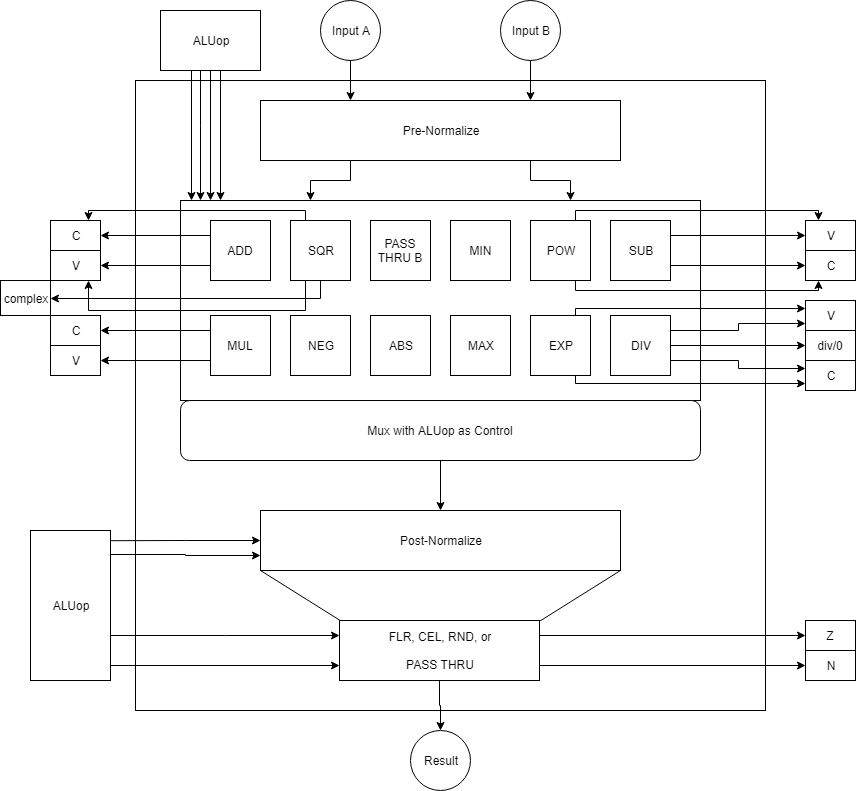
\includegraphics[width=1\linewidth]{ALUDesign.png}
\end{center}

\subsection{Datapath}
\subsubsection{Single Cycle}
\begin{center}
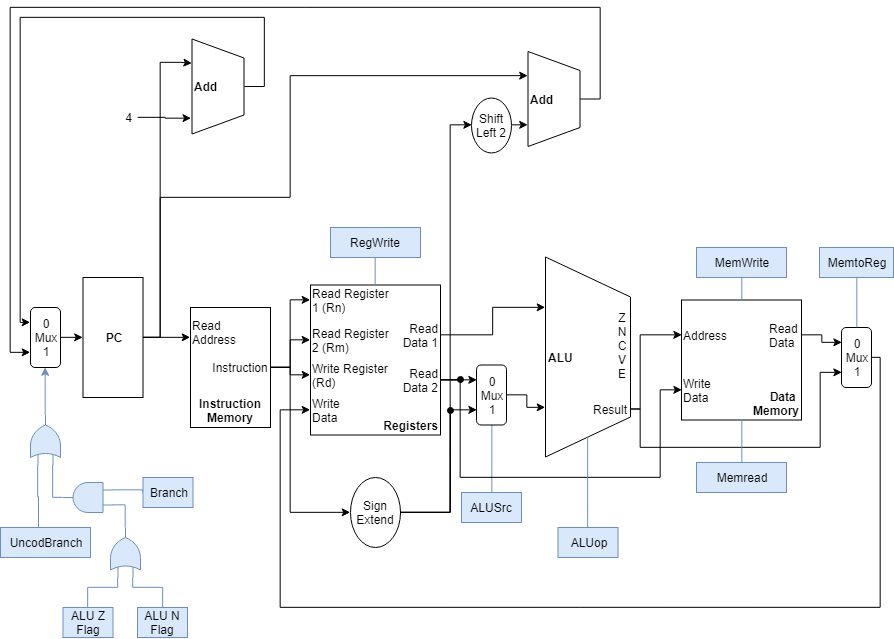
\includegraphics[width=1\linewidth]{SingleCycleArch.png}
\end{center}

\subsubsection{Pipelined}
\subsection{controller}

\begin{table}[!h]
\centering
\caption*{Datapath Control (We'll document what each of the signals means later, but its the same as the book)}
\begin{tabular}{lllllllll}
ASM & Opcode & ALUSrc & MemtoReg & RegWrite & MemRead & MemWrite & Branch & UncodBranch \\ \hline
\multicolumn{1}{|c|}{SET} & \multicolumn{1}{c|}{00000001} & \multicolumn{1}{c|}{1} & \multicolumn{1}{c|}{0} & \multicolumn{1}{c|}{1} & \multicolumn{1}{c|}{0} & \multicolumn{1}{c|}{0} & \multicolumn{1}{c|}{0} & \multicolumn{1}{c|}{0} \TBstrut \\[1em] \hline
\multicolumn{1}{|c|}{LOD} & \multicolumn{1}{c|}{00000010} & \multicolumn{1}{c|}{1} & \multicolumn{1}{c|}{1} & \multicolumn{1}{c|}{1} & \multicolumn{1}{c|}{1} & \multicolumn{1}{c|}{0} & \multicolumn{1}{c|}{0} & \multicolumn{1}{c|}{0} \TBstrut \\[1em] \hline
\multicolumn{1}{|c|}{STR} & \multicolumn{1}{c|}{00000011} & \multicolumn{1}{c|}{1} & \multicolumn{1}{c|}{X} & \multicolumn{1}{c|}{0} & \multicolumn{1}{c|}{0} & \multicolumn{1}{c|}{1} & \multicolumn{1}{c|}{0} & \multicolumn{1}{c|}{0} \TBstrut \\[1em] \hline

\multicolumn{1}{|c|}{MOV} & \multicolumn{1}{c|}{00000100} & \multicolumn{1}{c|}{0} & \multicolumn{1}{c|}{0} & \multicolumn{1}{c|}{1} & \multicolumn{1}{c|}{0} & \multicolumn{1}{c|}{0} & \multicolumn{1}{c|}{0} & \multicolumn{1}{c|}{0} \TBstrut \\[1em] \hline
\multicolumn{1}{|c|}{ADD} & \multicolumn{1}{c|}{00000101} & \multicolumn{1}{c|}{0} & \multicolumn{1}{c|}{0} & \multicolumn{1}{c|}{1} & \multicolumn{1}{c|}{0} & \multicolumn{1}{c|}{0} & \multicolumn{1}{c|}{0} & \multicolumn{1}{c|}{0} \TBstrut \\[1em] \hline
\multicolumn{1}{|c|}{SUB} & \multicolumn{1}{c|}{00000110} & \multicolumn{1}{c|}{0} & \multicolumn{1}{c|}{0} & \multicolumn{1}{c|}{1} & \multicolumn{1}{c|}{0} & \multicolumn{1}{c|}{0} & \multicolumn{1}{c|}{0} & \multicolumn{1}{c|}{0} \TBstrut \\[1em] \hline
\multicolumn{1}{|c|}{NEG} & \multicolumn{1}{c|}{00000111} & \multicolumn{1}{c|}{0} & \multicolumn{1}{c|}{0} & \multicolumn{1}{c|}{1} & \multicolumn{1}{c|}{0} & \multicolumn{1}{c|}{0} & \multicolumn{1}{c|}{0} & \multicolumn{1}{c|}{0} \TBstrut \\[1em] \hline
\multicolumn{1}{|c|}{MUL} & \multicolumn{1}{c|}{00001000} & \multicolumn{1}{c|}{0} & \multicolumn{1}{c|}{0} & \multicolumn{1}{c|}{1} & \multicolumn{1}{c|}{0} & \multicolumn{1}{c|}{0} & \multicolumn{1}{c|}{0} & \multicolumn{1}{c|}{0} \TBstrut \\[1em] \hline
\multicolumn{1}{|c|}{DIV} & \multicolumn{1}{c|}{00001001} & \multicolumn{1}{c|}{0} & \multicolumn{1}{c|}{0} & \multicolumn{1}{c|}{1} & \multicolumn{1}{c|}{0} & \multicolumn{1}{c|}{0} & \multicolumn{1}{c|}{0} & \multicolumn{1}{c|}{0} \TBstrut \\[1em] \hline
\multicolumn{1}{|c|}{FLR} & \multicolumn{1}{c|}{00001010} & \multicolumn{1}{c|}{0} & \multicolumn{1}{c|}{0} & \multicolumn{1}{c|}{1} & \multicolumn{1}{c|}{0} & \multicolumn{1}{c|}{0} & \multicolumn{1}{c|}{0} & \multicolumn{1}{c|}{0} \TBstrut \\[1em] \hline
\multicolumn{1}{|c|}{CEL} & \multicolumn{1}{c|}{00001011} & \multicolumn{1}{c|}{0} & \multicolumn{1}{c|}{0} & \multicolumn{1}{c|}{1} & \multicolumn{1}{c|}{0} & \multicolumn{1}{c|}{0} & \multicolumn{1}{c|}{0} & \multicolumn{1}{c|}{0} \TBstrut \\[1em] \hline
\multicolumn{1}{|c|}{RND} & \multicolumn{1}{c|}{00001100} & \multicolumn{1}{c|}{0} & \multicolumn{1}{c|}{0} & \multicolumn{1}{c|}{1} & \multicolumn{1}{c|}{0} & \multicolumn{1}{c|}{0} & \multicolumn{1}{c|}{0} & \multicolumn{1}{c|}{0} \TBstrut \\[1em] \hline
\multicolumn{1}{|c|}{ABS} & \multicolumn{1}{c|}{00001101} & \multicolumn{1}{c|}{0} & \multicolumn{1}{c|}{0} & \multicolumn{1}{c|}{1} & \multicolumn{1}{c|}{0} & \multicolumn{1}{c|}{0} & \multicolumn{1}{c|}{0} & \multicolumn{1}{c|}{0} \TBstrut \\[1em] \hline
\multicolumn{1}{|c|}{MIN} & \multicolumn{1}{c|}{00001110} & \multicolumn{1}{c|}{0} & \multicolumn{1}{c|}{0} & \multicolumn{1}{c|}{1} & \multicolumn{1}{c|}{0} & \multicolumn{1}{c|}{0} & \multicolumn{1}{c|}{0} & \multicolumn{1}{c|}{0} \TBstrut \\[1em] \hline
\multicolumn{1}{|c|}{MAX} & \multicolumn{1}{c|}{00001111} & \multicolumn{1}{c|}{0} & \multicolumn{1}{c|}{0} & \multicolumn{1}{c|}{1} & \multicolumn{1}{c|}{0} & \multicolumn{1}{c|}{0} & \multicolumn{1}{c|}{0} & \multicolumn{1}{c|}{0} \TBstrut \\[1em] \hline
\multicolumn{1}{|c|}{POW} & \multicolumn{1}{c|}{00010000} & \multicolumn{1}{c|}{0} & \multicolumn{1}{c|}{0} & \multicolumn{1}{c|}{1} & \multicolumn{1}{c|}{0} & \multicolumn{1}{c|}{0} & \multicolumn{1}{c|}{0} & \multicolumn{1}{c|}{0} \TBstrut \\[1em] \hline
\multicolumn{1}{|c|}{EXP} & \multicolumn{1}{c|}{00010001} & \multicolumn{1}{c|}{0} & \multicolumn{1}{c|}{0} & \multicolumn{1}{c|}{1} & \multicolumn{1}{c|}{0} & \multicolumn{1}{c|}{0} & \multicolumn{1}{c|}{0} & \multicolumn{1}{c|}{0} \TBstrut \\[1em] \hline
\multicolumn{1}{|c|}{SQR} & \multicolumn{1}{c|}{00010010} & \multicolumn{1}{c|}{0} & \multicolumn{1}{c|}{0} & \multicolumn{1}{c|}{1} & \multicolumn{1}{c|}{0} & \multicolumn{1}{c|}{0} & \multicolumn{1}{c|}{0} & \multicolumn{1}{c|}{0} \TBstrut \\[1em] \hline

\multicolumn{1}{|c|}{BRU} & \multicolumn{1}{c|}{00010011} & \multicolumn{1}{c|}{1} & \multicolumn{1}{c|}{X} & \multicolumn{1}{c|}{X} & \multicolumn{1}{c|}{X} & \multicolumn{1}{c|}{X} & \multicolumn{1}{c|}{X} & \multicolumn{1}{c|}{1} \TBstrut \\[1em] \hline
\multicolumn{1}{|c|}{BRZ} & \multicolumn{1}{c|}{00010100} & \multicolumn{1}{c|}{1} & \multicolumn{1}{c|}{X} & \multicolumn{1}{c|}{0} & \multicolumn{1}{c|}{0} & \multicolumn{1}{c|}{0} & \multicolumn{1}{c|}{1} & \multicolumn{1}{c|}{0} \TBstrut \\[1em] \hline
\multicolumn{1}{|c|}{BRN} & \multicolumn{1}{c|}{00010101} & \multicolumn{1}{c|}{1} & \multicolumn{1}{c|}{X} & \multicolumn{1}{c|}{0} & \multicolumn{1}{c|}{0} & \multicolumn{1}{c|}{0} & \multicolumn{1}{c|}{1} & \multicolumn{1}{c|}{0} \TBstrut \\[1em] \hline
\multicolumn{1}{|c|}{NOP} & \multicolumn{1}{c|}{00010110} & \multicolumn{1}{c|}{0} & \multicolumn{1}{c|}{0} & \multicolumn{1}{c|}{0} & \multicolumn{1}{c|}{0} & \multicolumn{1}{c|}{0} & \multicolumn{1}{c|}{0} & \multicolumn{1}{c|}{0} \TBstrut \\[1em] \hline
\multicolumn{1}{|c|}{HLT} & \multicolumn{1}{c|}{00010111} & \multicolumn{1}{c|}{0} & \multicolumn{1}{c|}{0} & \multicolumn{1}{c|}{0} & \multicolumn{1}{c|}{0} & \multicolumn{1}{c|}{0} & \multicolumn{1}{c|}{0} & \multicolumn{1}{c|}{0} \TBstrut \\[1em] \hline
\end{tabular}
\end{table}

\begin{table}[!h]
\centering
\caption*{ALU Control (ALUop)}
\begin{tabular}{llll}
ASM & Opcode & ALUop & Description \\ \hline
\multicolumn{1}{|c|}{SET} & \multicolumn{1}{c|}{00000001} & \multicolumn{1}{c|}{0000} & \multicolumn{1}{c|}{Pass Through} \TBstrut \\[1em] \hline
\multicolumn{1}{|c|}{LOD} & \multicolumn{1}{c|}{00000010} & \multicolumn{1}{c|}{0000} & \multicolumn{1}{c|}{Pass Through} \TBstrut \\[1em] \hline
\multicolumn{1}{|c|}{STR} & \multicolumn{1}{c|}{00000011} & \multicolumn{1}{c|}{0000} & \multicolumn{1}{c|}{Pass Through} \TBstrut \\[1em] \hline
\multicolumn{1}{|c|}{MOV} & \multicolumn{1}{c|}{00000100} & \multicolumn{1}{c|}{0000} & \multicolumn{1}{c|}{Pass Through} \TBstrut \\[1em] \hline 
\multicolumn{1}{|c|}{ADD} & \multicolumn{1}{c|}{00000101} & \multicolumn{1}{c|}{0001} & \multicolumn{1}{c|}{Use Adder} \TBstrut \\[1em] \hline
\multicolumn{1}{|c|}{SUB} & \multicolumn{1}{c|}{00000110} & \multicolumn{1}{c|}{0010} & \multicolumn{1}{c|}{Use Subtracter} \TBstrut \\[1em] \hline
\multicolumn{1}{|c|}{NEG} & \multicolumn{1}{c|}{00000111} & \multicolumn{1}{c|}{0011} & \multicolumn{1}{c|}{Negate} \TBstrut \\[1em] \hline
\multicolumn{1}{|c|}{MUL} & \multicolumn{1}{c|}{00001000} & \multicolumn{1}{c|}{0100} & \multicolumn{1}{c|}{Use Multiplier} \TBstrut \\[1em] \hline
\multicolumn{1}{|c|}{DIV} & \multicolumn{1}{c|}{00001001} & \multicolumn{1}{c|}{0101} & \multicolumn{1}{c|}{Use Divider} \TBstrut \\[1em] \hline
\multicolumn{1}{|c|}{FLR} & \multicolumn{1}{c|}{00001010} & \multicolumn{1}{c|}{0110} & \multicolumn{1}{c|}{Floor Result} \TBstrut \\[1em] \hline
\multicolumn{1}{|c|}{CEL} & \multicolumn{1}{c|}{00001011} & \multicolumn{1}{c|}{0111} & \multicolumn{1}{c|}{Ceil Result} \TBstrut \\[1em] \hline
\multicolumn{1}{|c|}{RND} & \multicolumn{1}{c|}{00001100} & \multicolumn{1}{c|}{1000} & \multicolumn{1}{c|}{Round Result} \TBstrut \\[1em] \hline
\multicolumn{1}{|c|}{ABS} & \multicolumn{1}{c|}{00001101} & \multicolumn{1}{c|}{1001} & \multicolumn{1}{c|}{Take Absolute Value} \TBstrut \\[1em] \hline
\multicolumn{1}{|c|}{MIN} & \multicolumn{1}{c|}{00001110} & \multicolumn{1}{c|}{1010} & \multicolumn{1}{c|}{Take Minimum Input} \TBstrut \\[1em] \hline
\multicolumn{1}{|c|}{MAX} & \multicolumn{1}{c|}{00001111} & \multicolumn{1}{c|}{1011} & \multicolumn{1}{c|}{Take Maximum Input} \TBstrut \\[1em] \hline
\multicolumn{1}{|c|}{POW} & \multicolumn{1}{c|}{00010000} & \multicolumn{1}{c|}{1100} & \multicolumn{1}{c|}{Take Power} \TBstrut \\[1em] \hline
\multicolumn{1}{|c|}{EXP} & \multicolumn{1}{c|}{00010001} & \multicolumn{1}{c|}{1101} & \multicolumn{1}{c|}{Exponentiate} \TBstrut \\[1em] \hline
\multicolumn{1}{|c|}{SQR} & \multicolumn{1}{c|}{00010010} & \multicolumn{1}{c|}{1110} & \multicolumn{1}{c|}{Take Square Root} \TBstrut \\[1em] \hline
\multicolumn{1}{|c|}{BRU} & \multicolumn{1}{c|}{00010011} & \multicolumn{1}{c|}{0000} & \multicolumn{1}{c|}{Pass Through} \TBstrut \\[1em] \hline
\multicolumn{1}{|c|}{BRZ} & \multicolumn{1}{c|}{00010100} & \multicolumn{1}{c|}{0000} & \multicolumn{1}{c|}{Pass Through} \TBstrut \\[1em] \hline
\multicolumn{1}{|c|}{BRN} & \multicolumn{1}{c|}{00010101} & \multicolumn{1}{c|}{0000} & \multicolumn{1}{c|}{Pass Through} \TBstrut \\[1em] \hline
\multicolumn{1}{|c|}{NOP} & \multicolumn{1}{c|}{00010110} & \multicolumn{1}{c|}{0000} & \multicolumn{1}{c|}{Pass Through} \TBstrut \\[1em] \hline
\multicolumn{1}{|c|}{HLT} & \multicolumn{1}{c|}{00010111} & \multicolumn{1}{c|}{0000} & \multicolumn{1}{c|}{Pass Through} \TBstrut \\[1em] \hline
\end{tabular}
\end{table}

\section{VHDL Description}
\section{Testing}
\section{Conclusion}
\end{document}